\documentclass{beamer}
\usetheme{default}

\usepackage{caption}
\usepackage{subcaption}

\title{title}
\author{T.\ Northey}
\begin{document}
\begin{frame}[plain]
    \maketitle
\end{frame}

\begin{frame}{Defining structure pool parameters}
\begin{center}
	{\huge$\mu$}\qquad\qquad{\huge$\sigma_i$}\\
	\vspace{2cm}
	{\huge$\rho$}
\end{center}
\end{frame}

\begin{frame}{Defining structure pool parameters}
	\begin{center}

	\end{center}
\end{frame}

\begin{frame}{Defining structure pool parameters}
		\begin{center}
	{\huge$\mu=0$, e.g.\ $\textbf{R}_0$}
		\end{center}
	
	[picture of potential energy curve along a bond-distance, + bell curve vibrational distribution]
	
	[and picture of $\mu\neq 0$ situation, shifted bell curve]
\end{frame}

\begin{frame}{Defining structure pool parameters}
		\begin{center}
	$\sigma=\begin{pmatrix}
	0.4 \\
	0.2\\
	0.2\\
	\vdots\\
	0.2
	\end{pmatrix}
	$ \AA
		\end{center}
	
	\begin{itemize}
		\item some displacements more important than others
		\item some could be irrelevant $\sigma_i = 0$ (i.e.\ don't displace at all)
	\end{itemize}

\end{frame}

\begin{frame}{Defining structure pool parameters}
		\begin{center}
	\qquad\qquad\qquad\ \ \ {\huge$\rho\propto\textrm{accuracy / resolution}$}\\
		\vspace{2mm}
	{\huge$\propto N$}\\
		\vspace{2mm}
	\quad\ \ {\huge$\propto 1/\sigma_i$}\\
	%\qquad\qquad\qquad\ \ {\huge$\propto 1/n_{\textrm{modes}}$}\\

		\end{center}

\end{frame}

\begin{frame}{NMM previous work}
	\begin{figure}[H]
	\centering
		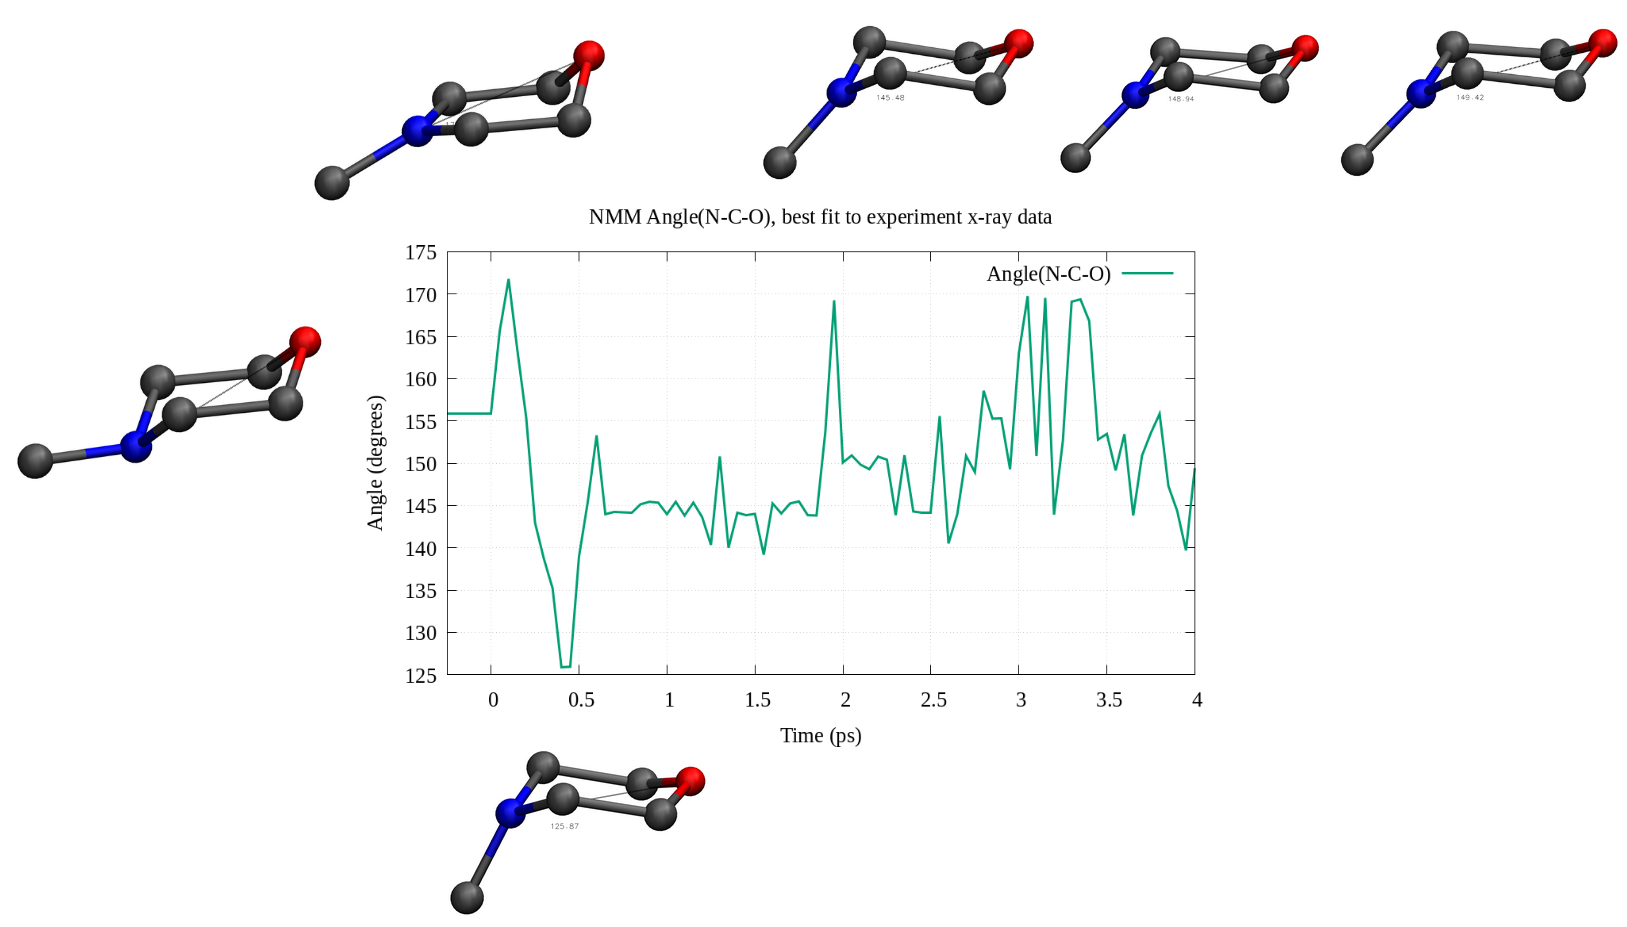
\includegraphics[width=\textwidth]{geomovie_ppt_slide.png}
		\caption{N-C-O angle of best fit to experiment trajectory.}
		\label{fig:geomovie-ppt-slide}
	\end{figure}
	
\end{frame}


\begin{frame}{Sampling method}
The sampling equation for generating the displaced molecular coordinates is,

\begin{eqnarray}
\textbf{R} = \textbf{R}_0 + \sum_i^{\textrm{modes}} a_i\textbf{d}_i
\end{eqnarray}

with starting geometry $\textbf{R}_0$, and displacement unit vectors $\textbf{d}_i$ for each normal mode are obtained from a frequency calculation.  The factors $a_i$ are randomly generated within a bell curve centered at $\mu=0$, and chosen standard deviation, $\sigma$. 
\end{frame}


\end{document}
